\chapter{Implementation}
\label{sec:implementation}

Hardware Architecture

The HWFRA architecture is composed by 4 component: Server state machine, Client state machine, Scheduler and Switcher.
All AXIS Stream input and output signals from heterogeneous nodes connected to the Switcher and all scheduler control signals and actionlib control signals connect to the Scheduler module.

Max component can find out the maximum number and its index of the given list. The max component output the max number in the input list and the index of the max data in less than 1 clock.

\section{Max}

Max component has a binary tree structure like many other compare circuits of a 2-compare sub-component vector, but each basic  compare block output the bigger number and a bit to indicate which side is bigger. ‘1’ for the left number is bigger and ‘0’ means the right one is bigger.
We build a compare result table to indicate if each number is bigger in the compare in this round. If a data got ‘1’ in all the compares, than its the biggest number.

Formula 6.1 shows that which output bit in the 2 compare sub-component vector is related to the value of the compare result table. Formula 6.2 compute the bit from index computed in Formula 6.1 should be taken a not function.

let RI, IB functions of a integer, where RI means Related index, and IB = means Is bigger. We define the functions as following: 

$
 IP(i) =\lfloor \frac{\lfloor\frac{i}{r} \rfloor}{2^{i \bmod r + 1}  }\rfloor + 2^{( r -1 - i \bmod r)}
$


% \begin{table}[htb]
% 	\centering
% 	\caption{Related Index Table for 4 Inputs}
% 	\begin{tabular}{l c}
% 		\toprule
% 		Round  & index \\ \midrule
% 		Round 1 &  2, 1, 2, 1 \\
% 		Round 2 &  3, 1, 3, 1  \\
% 		\bottomrule
% 	\end{tabular}
% 	\label{tab:flocklab_clock_offset}
% \end{table}

\begin{table}[htb]
	\centering
	\caption{Related Index Table for 8 Inputs}
	\begin{tabular}{l c c c}
		\toprule
		Input  & Round1  & Round2  & Round3 \\ \midrule
		Input 0 &  4& 2& 1\\
		Input 1 & 4& 2& 1  \\
		Input 2 & 5& 2&   1\\
	        Input 3 & 5& 2& 1\\
	        Input 4 & 6& 3& 1\\
		Input 5 & 6&  3& 1\\
		Input 6 & 7& 3& 1\\
		Input 7 & 7& 3& 1  \\
		\bottomrule
	\end{tabular}
	\label{tab:max-step1}
\end{table}


$
 IB(i) = \lfloor\frac{i}{r} \rfloor \bmod 2 ^{ i \bmod r + 1} < 2 ^{ i \bmod r}
$

\begin{table}[htb]
	\centering
	\caption{Is Bigger Table for 8 Inputs}
	\begin{tabular}{l c c c}
		\toprule
		Input  & Round1  & Round2  & Round3 \\ \midrule
		Input 0 &  False& False& False\\
		Input 1 &  True & False& False  \\
		Input 2 & False& True&  False\\
	    Input 3 & True& True& False\\
	    Input 4 & False& False& True\\
		Input 5 & True&  False& True\\
		Input 6 & False& True&True\\
		Input 7 & True& True& True  \\
		\bottomrule
	\end{tabular}
	\label{tab:max-step2}
\end{table}

Here round means the total layer of the compare process and equal to ceil of the data count. The computed tables is a constant to each round number. Therefore the computation is done in compile time and won't add to the hardware architecture complexity.
Replace the index of the Related Index Table with the corresponding compare result signal from compare component list, the xor the result with Is bigger Table, the result is one hot vector of the bit-wise-and of r rows of the new table.
 The basic idea is like finding the winner of a championship match table, you need to check all game of a player, and he is the final winner if all the games is won. Here, the IP function means to find all the games result of the player, and for compare result '1' means the left player won, IB means if the player is on the left side. 
 
 \begin{table}[htb]
	\centering
	\caption{Example and Explanation }
	\begin{tabular}{l c c c}
		\toprule
		I/O  & Input  & Max  & Index \\ \midrule
		Example  &  0x34605721& 0x7& 00000100\\
		Explanation  & number list  & max input& max number at position 5  \\
		\bottomrule
	\end{tabular}
	\label{tab:max}
\end{table}
 
 \begin{figure}[htb]
	\centering
	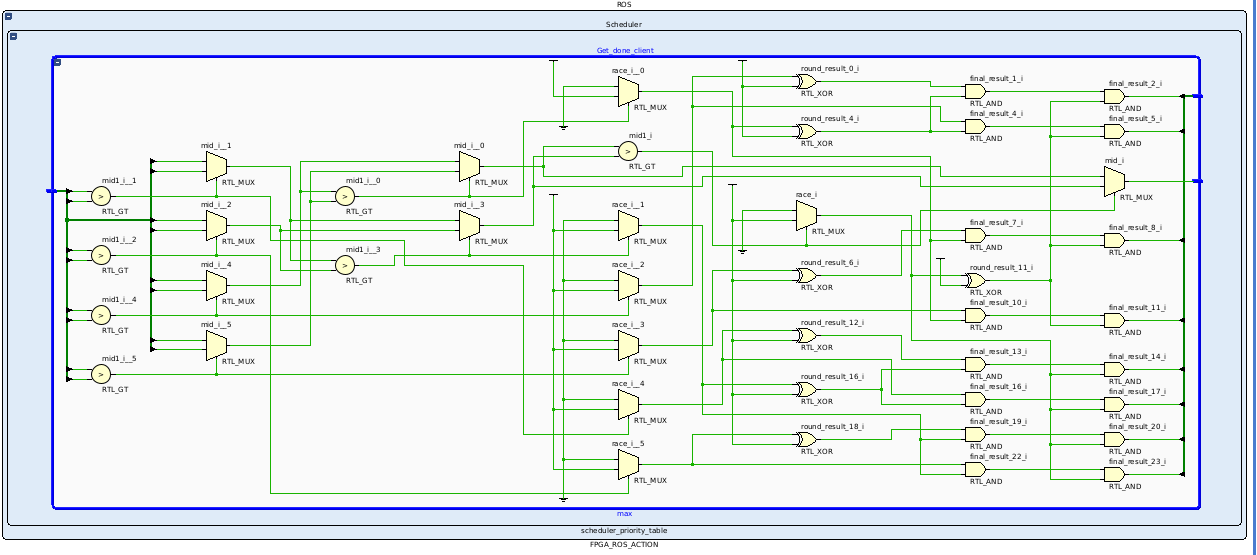
\includegraphics[width=.8\linewidth]{figures/max8.png}
	\caption{Max Component Design}
	\label{fig:max}
\end{figure}
 
\section{Min}

Min component can find out the minimum number and its index of the given list. Min component is the same like the Max component, except all greater than compare are substituted by less than compares.

 \begin{table}[htb]
	\centering
	\caption{Example and Explanation }
	\begin{tabular}{l c c c}
		\toprule
		I/O  & Input  & Min  & Index \\ \midrule
		Example  &  0x34605721& 0x0& 00010000\\
		Explanation  & number list  & min input& min number at position 3  \\
		\bottomrule
	\end{tabular}
	\label{tab:tab-min}
\end{table}

 \begin{figure}[htb]
	\centering
	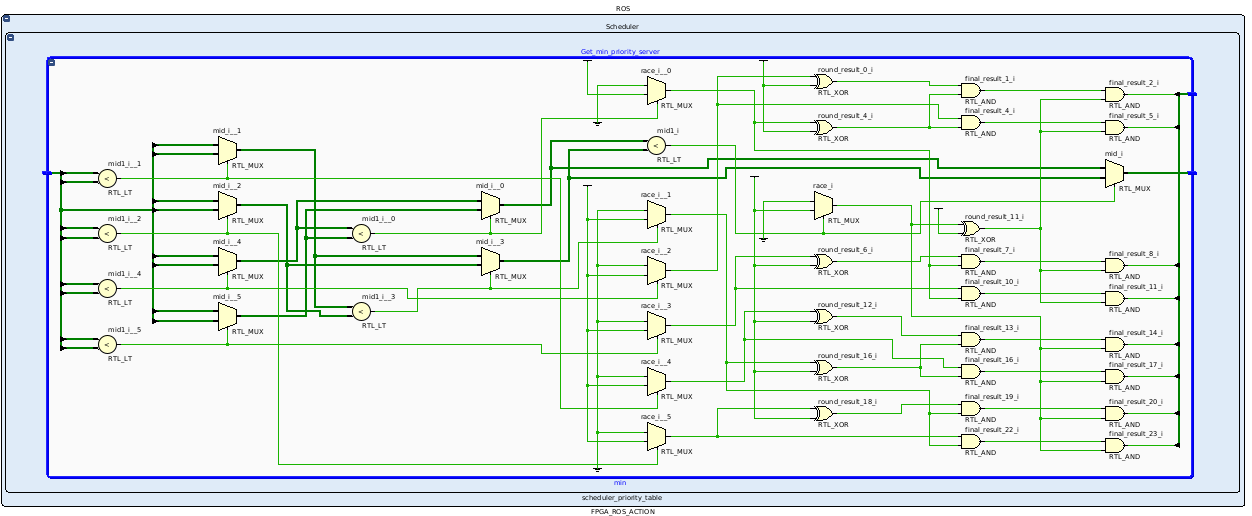
\includegraphics[width=.8\linewidth]{figures/min8.png}
	\caption{Min Component Design}
	\label{fig:min}
\end{figure}
 


The min component output the min number in the input list and the index of the min data in less than 1s.

\section{One Hot to Unsigned}

This component can convert one hot vector to a compact unsigned integer. One hot vector means a signal vector with exactly one signal is ‘1’ and all other signals are ‘0’.

 \begin{table}[htb]
	\centering
	\caption{Example and Explanation }
	\begin{tabular}{l c c}
		\toprule
		I/O  &  One-hot  & Index \\ \midrule
		Example  &  00010000 & 3\\
		Explanation  & Only the 4th bit is '1'  & Index of '1'  \\
		\bottomrule
	\end{tabular}
	\label{tab:tab-o2n}
\end{table}
%   tree:    for j in MAX/2-1 downto 1 generate
%         selection(j) <= '1'  when  selection (2 * j) = '1' else
%                         '1'  when  selection (2 * j + 1) = '1'  else  '0';   
%         position(j)  <=  position(j-1) when selection(j) = '0' else
%                         '0'  when  selection(j) = '1' and selection (2 * j) = '1' else
%                         '1'  when  selection(j) = '1' and selection (2 * j + 1) = '1'  else  'X';   
%     end generate;
%     leaf:    for j in MAX/2 -1 downto 0 generate
%         selection(j + MAX/2) <=   '1'    when i(2 * j) = '1' else
%                                   '1'    when i(2 * j + 1) = '1' else '0'; 
%         position(j + MAX/2)  <=   position(j-1+MAX/2) when selection(j + MAX/2) = '0' else
%                                   '0'    when i(2 * j) = '1' else
%                                   '1'    when i(2 * j + 1) = '1' else '0';   
%     end generate;
%     result:    for j in LOG downto 1 generate
%         o(LOG-j) <= position(2**j-1);
         \begin{figure}[htb]
	\centering
	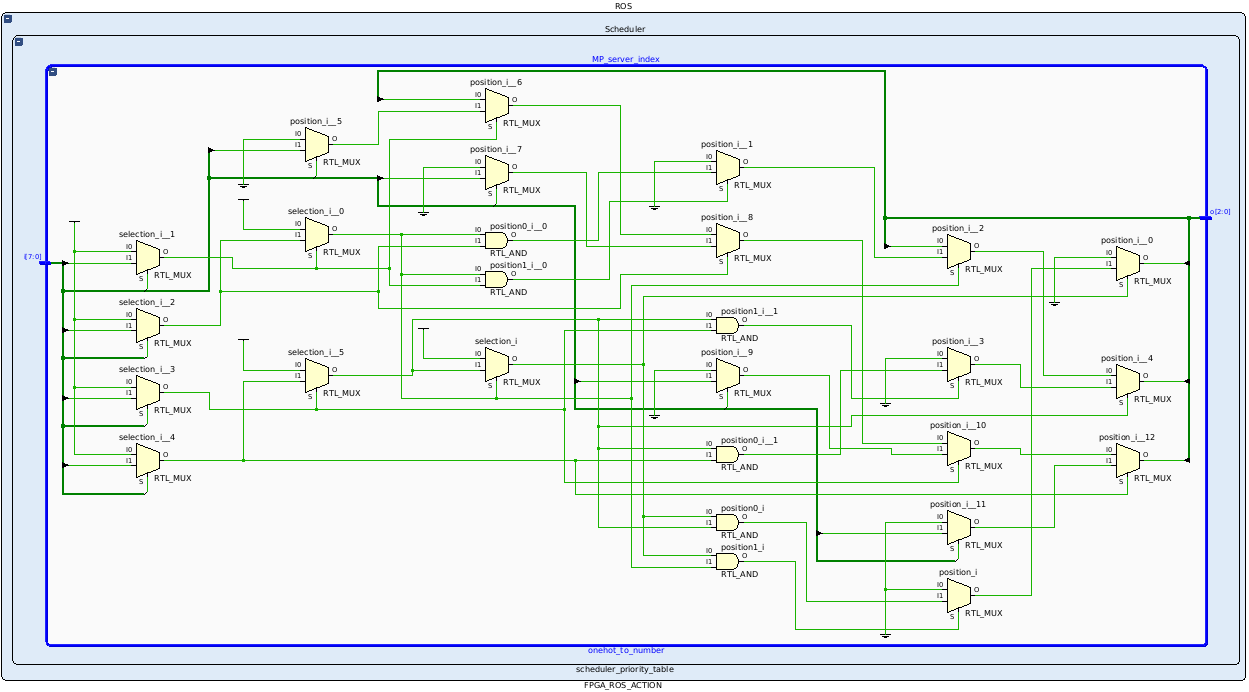
\includegraphics[width=.8\linewidth]{figures/o2n.png}
	\caption{One Hot to Unsigned Component Design}
	\label{fig:o2n}
\end{figure}
 
\section{Generic MUX}

	This component uses the VHDL generic technique and binary tree indexing to generalize a multiplexer for any number of input with any number of data width.
	
 \begin{table}[htb]
	\centering
	\caption{Example and Explanation }
	\begin{tabular}{l c c c}
		\toprule
		I/O  &  Input  & Selector & Result \\ \midrule
		Example  &  0x34605721 & 3 & 0\\
		Explanation  & 8 Input number with 4 bits each \\
		\bottomrule
	\end{tabular}
	\label{tab:tab-mux}
\end{table}	
	
\begin{figure}[htb]
	\centering
	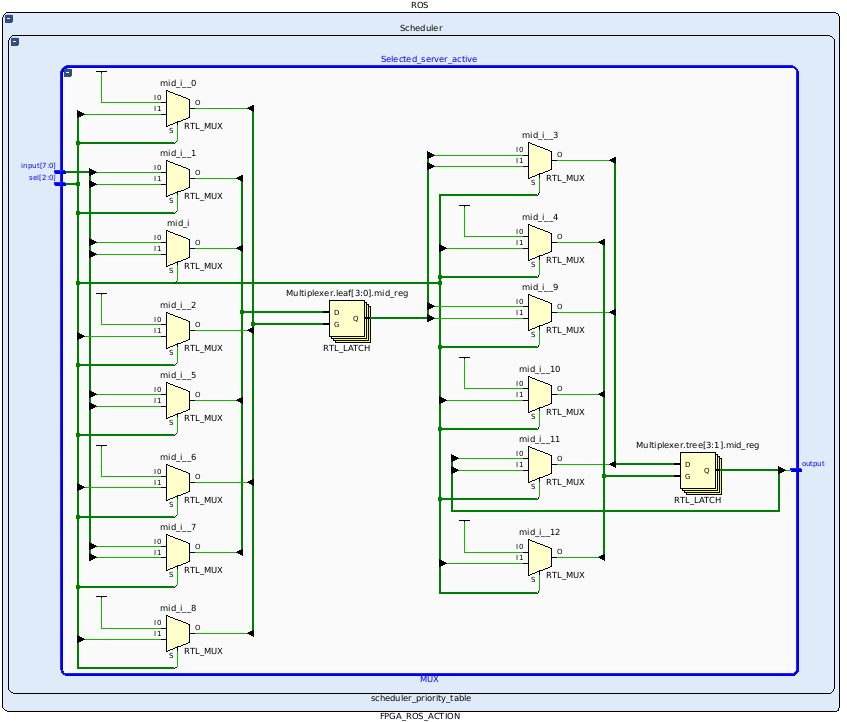
\includegraphics[width=.8\linewidth]{figures/mux.png}
	\caption{Generic MUX Component Design}
	\label{fig:mux}
\end{figure}
 
\section{Generic MUX with switch}

	This component add a ready flag bit vector as input to a generic MUX. If the ready bit of the selected data is ‘0’, then it output all zero, else it output the selected data.
	
\begin{table}[htb]
	\centering
	\caption{Example and Explanation }
	\begin{tabular}{l c c c c}
		\toprule
		I/O  &  Input  & Selector & Switch & Result \\ \midrule
		Example  &  0x34605721 & 3 & '0' & 0x0\\
		Explanation  & Set switch to '0', result will be all zero.\\
		\bottomrule
	\end{tabular}
	\label{tab:muxpp}
\end{table}		
	
\begin{figure}[htb]
	\centering
	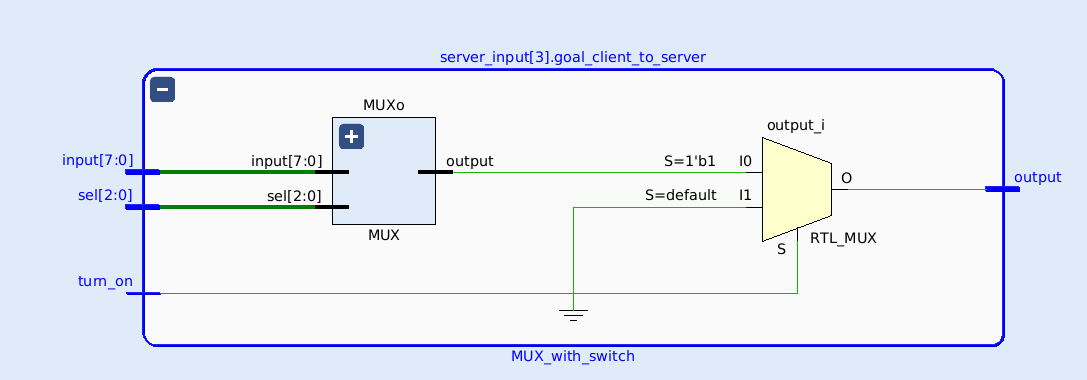
\includegraphics[width=.5\linewidth]{figures/mux-w-s.png}
	\caption{Generic MUX with switch Component Design}
	\label{fig:muxpp}
\end{figure}
\section{Signal Register}
 
	This component is designed for save signal that not hold. For example, the AXIS Stream tlast is set only at the last bit of transmission. If we want to use the this signal as a finish control signal to adapt AXIS Stream architectures seamlessly, we have to add a register to hold its value.
\begin{figure}[htb]
	\centering
	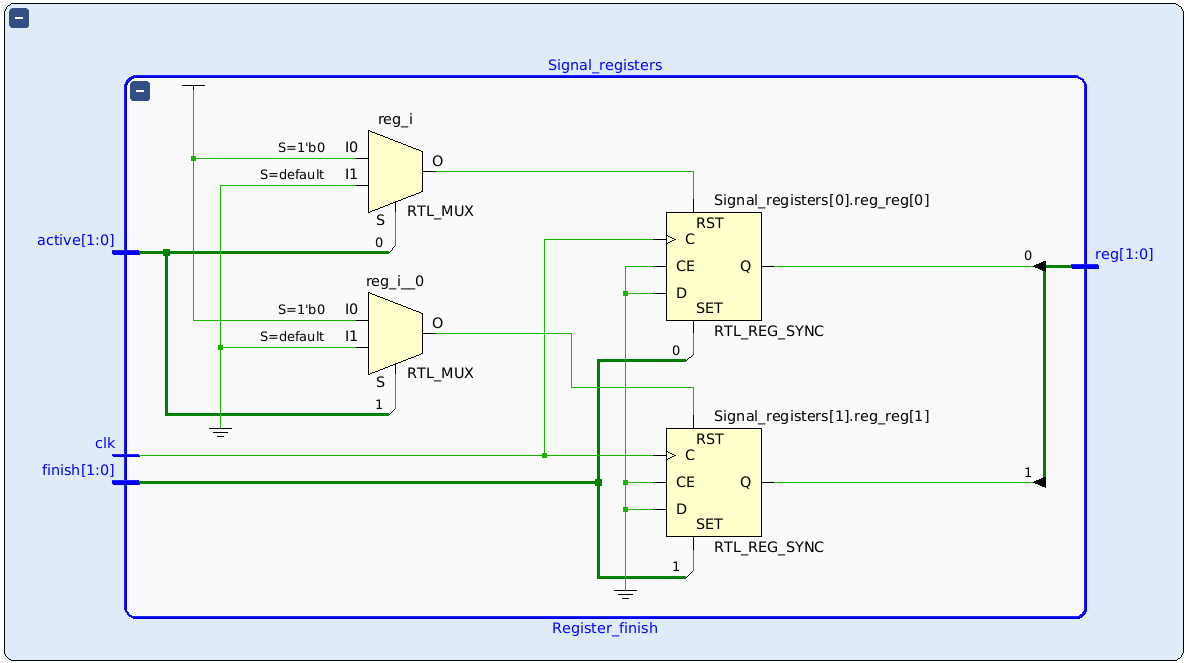
\includegraphics[width=.8\linewidth]{figures/Signal-reg.png}
	\caption{Generic MUX with switch Component Design}
	\label{fig:sigreg}
\end{figure}	

\section{Atomic Client Server Register}

    This register holds the scheduler information for all nodes, including client and server nodes. One server can serve only one client at the same time. The id of its serving client is stored in the register and if the active flag is active, then the id is valid. This the the same for clients and the connection state of a client and a server is added, changed or removed atomically.
    
     \begin{table}[htb]
	\centering
	\caption{Example for Client Register }
	\begin{tabular}{l c c}
		\toprule
		I/O  & Server  & Active \\ \midrule
		Client0  &  0x0 & '0'\\
		Client1  &  0x3 & '1'\\
		Client2  &  0x3 & '0'\\
		Client3  &  0x2 & '1'\\	
		\bottomrule
	\end{tabular}
	\label{tab:csreg}
\end{table}

     \begin{table}[htb]
	\centering
	\caption{Example for Server Register }
	\begin{tabular}{l c c}
		\toprule
		I/O  & Client  & Active \\ \midrule
		Server0  &  0x0 & '0'\\
		Server1  &  0x1 & '0'\\
		Server2  &  0x3 & '1'\\
		Server3  &  0x2 & '1'\\	
		\bottomrule
	\end{tabular}
	\label{tab:csreg2}
\end{table}

\begin{figure}[htb]
	\centering
	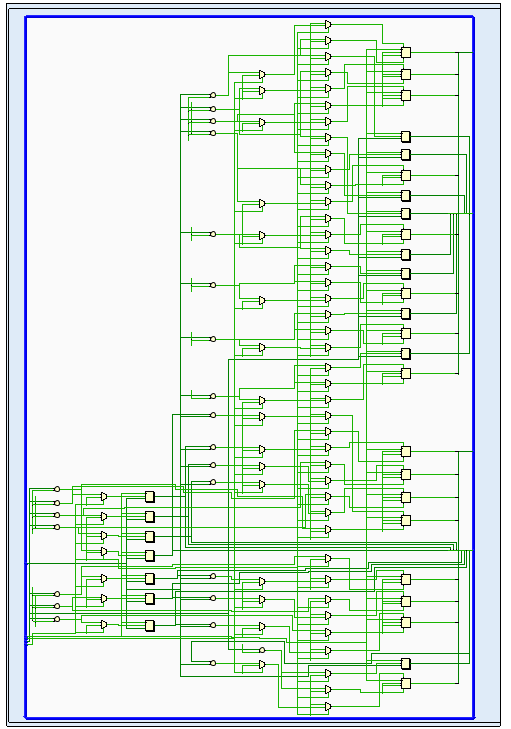
\includegraphics[width=.8\linewidth]{figures/atomic-reg.png}
	\caption{Atomic C/S Register Component Design}
	\label{fig:csreg}
\end{figure}


\section{Priority Table}

This register holds all priority numbers of clients and servers. The max priority number of ready clients and servers and their index will be found and then the client and server will be write into atomic client server register.
         \begin{table}[htb]
	\centering
	\caption{Example for Priority Register }
	\begin{tabular}{l c c}
		\toprule
		I/O  & Priority  & Ready \\ \midrule
		Server0  &  0x0 & '0'\\
		Server1  &  0x1 & '0'\\
		Server2  &  0x3 & '1'\\
		Server3  &  0x2 & '1'\\
		Client0   &  0x0 & '0'\\
		Client1   &  0x1 & '0'\\
		Client2   &  0x3 & '1'\\
		Client3   &  0x2 & '1'\\	
		\bottomrule
	\end{tabular}
	\label{tab:pri-tab}
\end{table}

\section{Switch}

This switch design connect each client node to all the server nodes. Each client node has its own circuit to listen to the change of its register in the atomic client server table. This is a simple topology to make sure every client can connected to the correspondent server as soon as possible.

\begin{figure}[htb]
	\centering
	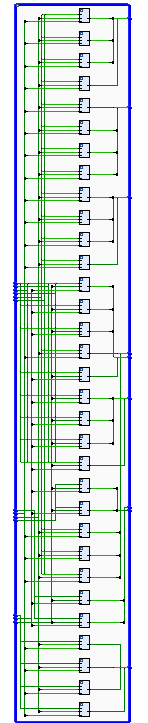
\includegraphics[width=.25\linewidth]{figures/new-sim/switch.png}
	\caption{Switch}
	\label{fig:switch}
\end{figure}

\section{Test Client}

This paper has also implemented a test client that implemented a subset of ROS actionlib framework design. This test client read a input file from simulator host operating system, Linux or Windows, generate a list of goals according to the input and wait to receive a result. When all goals are served, it write a output data and quit.

The goal data structure is an single 32 bit integer.
\begin{figure}[htb]
	\centering
	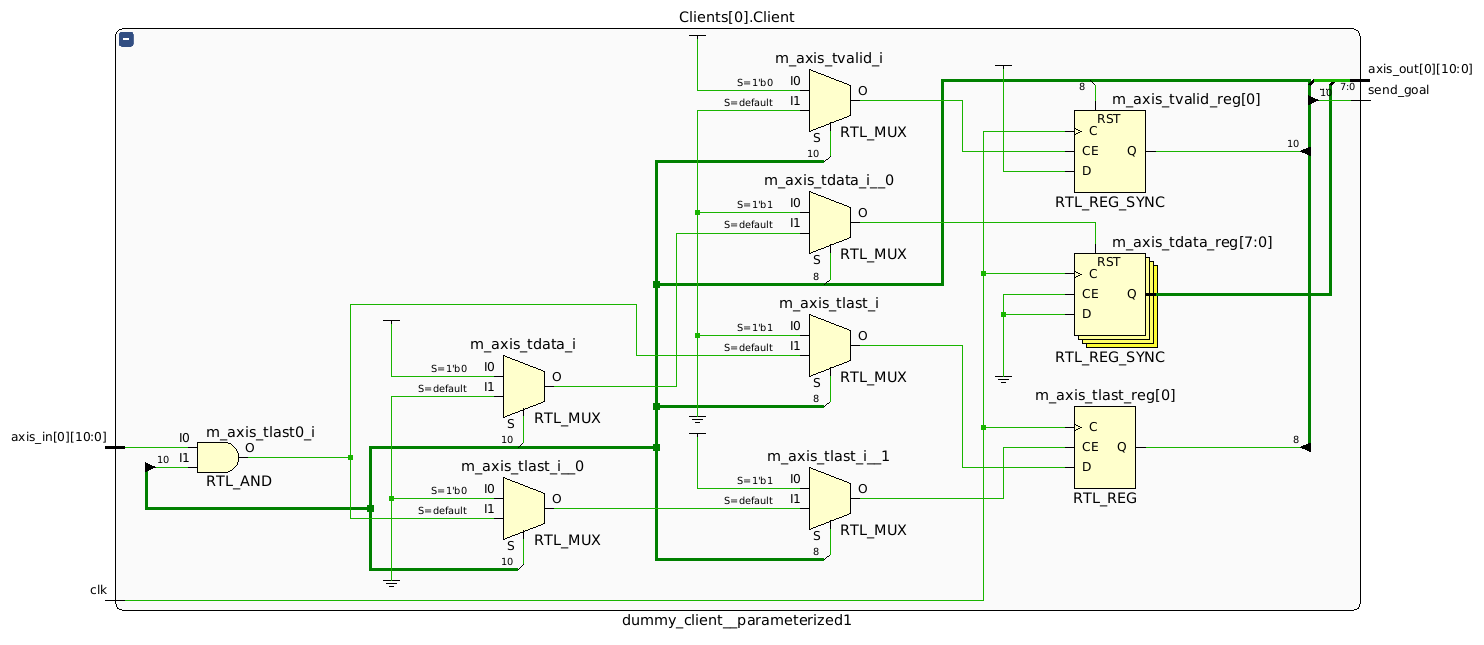
\includegraphics[width=.8\linewidth]{figures/Client.png}
	\caption{Test Client Design}
	\label{fig:client-tb}
\end{figure}
\section{Test Server}

Test server implemented a Fibonacci function to test the functionality of the HWFRA design. After received a 32 bit integer number goal from its input AXIS Stream port, it return the number of the Fibonacci sequence at that position as a 32 bit integer.
\begin{figure}[htb]
	\centering
	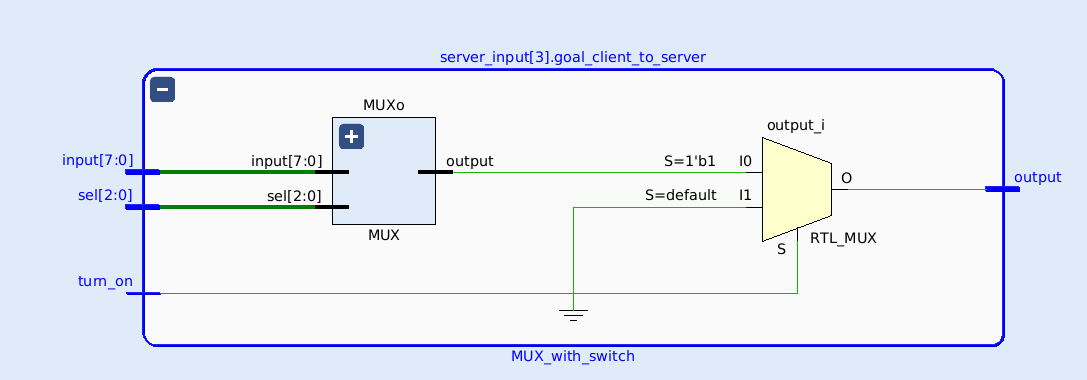
\includegraphics[width=.8\linewidth]{figures/mux-w-s.png}
	\caption{Generic MUX with switch Component Design}
	\label{fig:server-tb}
\end{figure}
\section{Scheduler: Round Robin }

This scheduler part implemented the simplest scheduler policy round robin. It checks all the clients if it is ready in turn. If a ready client is ready, then it check all the servers in turn to find a available one.

Note this implementation don't use priority table system described above and is not fully combinational. It takes in worst case number of clients -1 clock cycle to decide next client and number of servers -1 clock cycle to find a server.

It is possible to reduce worst case time to 1 circle by using the priority table system provided above by letting each client/server priority increase by 1 and reset to 0 if it reaches number of client/server.

\begin{figure}[htb]
	\centering
	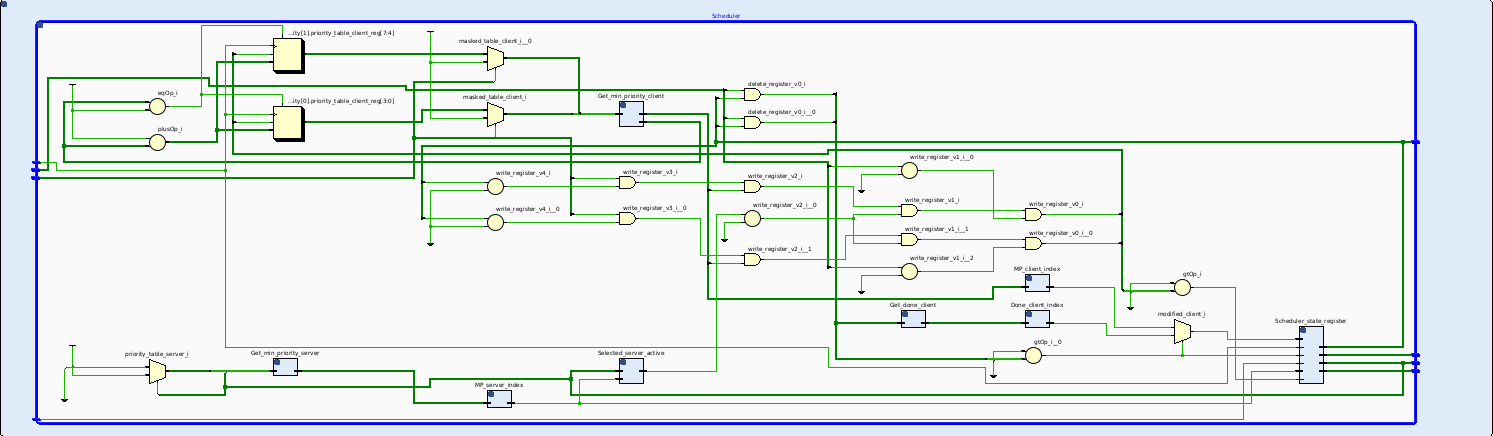
\includegraphics[width=.8\linewidth]{figures/Scheduler.png}
	\caption{Scheduler Design Round Robin}
	\label{fig:schedulerRR}
\end{figure}


\section{Scheduler: Least Recent Used}

The scheduler read the priority table for the lowest priority number and hold a max signal, if a node is used, then its priority will be set to max priority + 1.

If the max reach the max capacity of the priority number width, which is 255 for width equals 8, reset all priority number to 0.

\begin{figure}[htb]
	\centering
	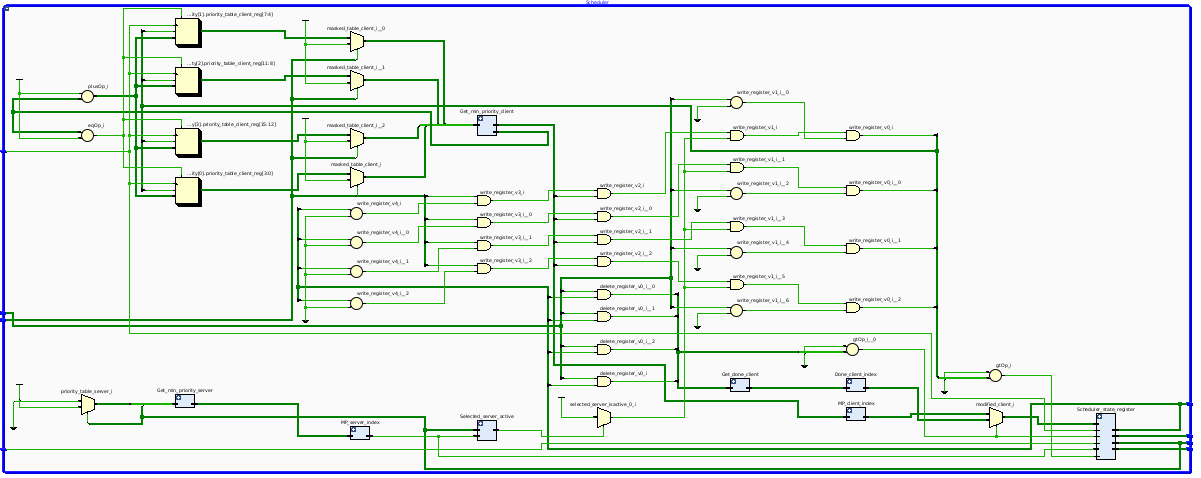
\includegraphics[width=.8\linewidth]{figures/new-sim/scheduler.png}
	\caption{Scheduler Design LRU}
	\label{fig:schedulerLRU}
\end{figure}


\section{Scheduler: Least frequent Used}

The scheduler read the priority table for the lowest priority number, if a node is used, then its priority will be set to its priority number + 1.

If the max reach the max capacity of the priority number width, which is 255 for width equals 8, reset all priority number to 0.
